\subsection{Bot Telegram}
	La componente \textit{bot Telegram} permette di ricevere codici di autenticazione a due fattori, notifiche di alert ed inviare direttamente dei comandi ai singoli dispositivi, per alterarne lo stato.
	\newline
	La componente è stata sviluppata usando JavaScript ed i moduli Axios, HTTP e Telegraf.
	 
\subsubsection{Diagramma delle classi}%%%%%%%%%%%%%%%%%OK
	\begin{figure}[H]
		\centering
		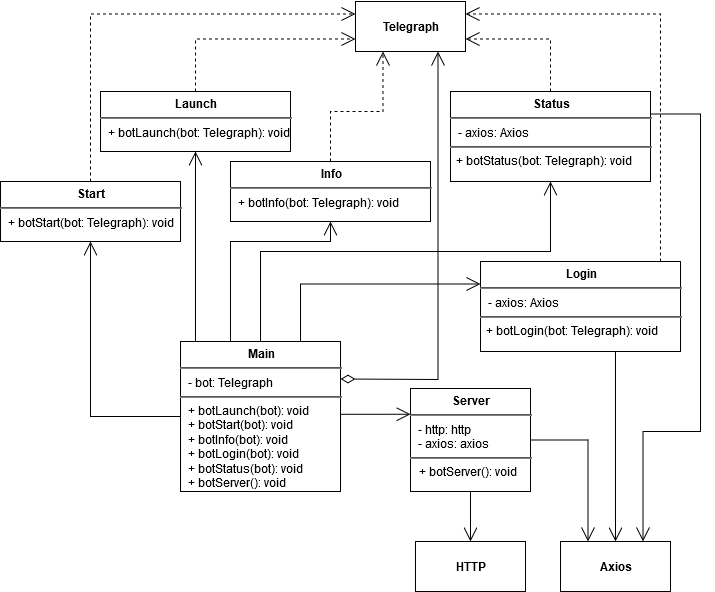
\includegraphics[scale=0.600]{res/images/BOTTELEGRAM/ClassiTelegram.png}
		\caption{Diagramma delle classi della componente bot Telegram}
		\label{Diagramma 19}
	\end{figure}
\subsubsection{Diagramma di sequenza}%%%%%%%%%OK
	\begin{figure}[H]
		\centering
		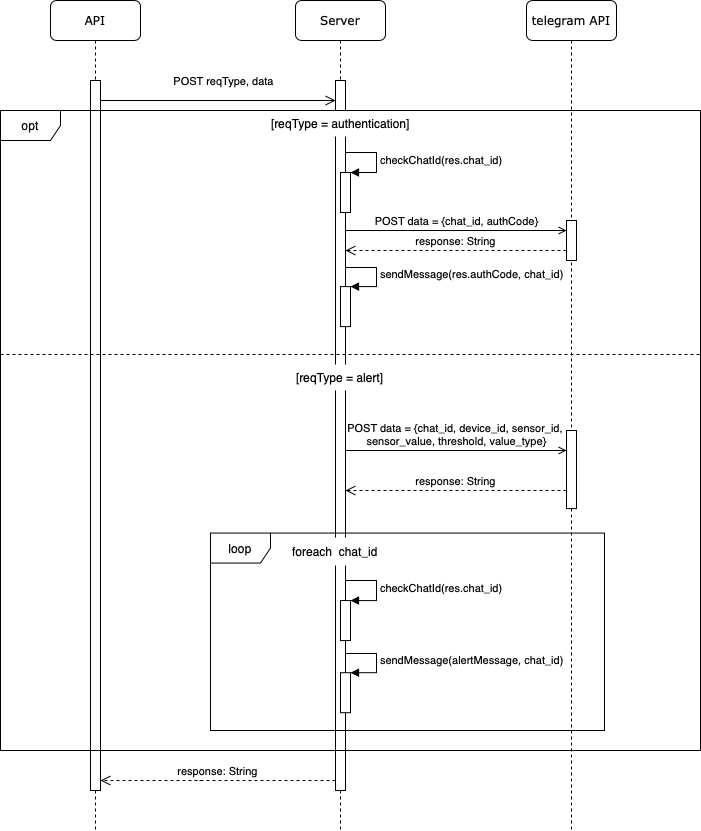
\includegraphics[scale=0.600]{res/images/BOTTELEGRAM/TelegramRichiestaPOST.png}
		\caption{Diagramma di sequenza che riporta la ricezione di una richiesta POST delle api all'interno della componente bot Telegram}
		\label{Diagramma 20}
	\end{figure}